\documentclass[11pt]{article}
\usepackage[T1]{fontenc}
\usepackage{lmodern,amsmath,amssymb}
\usepackage[margin=25mm]{geometry}
\usepackage{graphicx,float}
\usepackage{longtable,booktabs,array}
\usepackage{xcolor}
\usepackage[unicode]{hyperref}
\usepackage{xurl}
\hypersetup{pdfauthor={Eduardo Arana},pdftitle={Shared UI State and Host
Enforcement: An Empirical Technical Note on Three Agent-UI
Configurations},colorlinks=true,allcolors=black}
\urlstyle{same}
\setcounter{secnumdepth}{3}
\setlength{\parindent}{1em}
\setlength{\parskip}{2pt}
\setlength{\emergencystretch}{3em}
\setlength{\LTpre}{6pt}
\setlength{\LTpost}{6pt}
\newcounter{none}
\providecommand{\tightlist}{\setlength{\itemsep}{0pt}\setlength{\parskip}{0pt}}
\newcommand{\pandocbounded}[1]{#1}
\renewcommand{\topfraction}{0.9}
\renewcommand{\bottomfraction}{0.8}
\renewcommand{\textfraction}{0.05}
\renewcommand{\floatpagefraction}{0.85}
\title{Shared UI State and Host Enforcement: An Empirical Technical Note
on Three Agent-UI Configurations}
\author{Eduardo Arana}
\date{Independent researcher\\[4pt]26 September 2026}
\begin{document}
\special{pdf:minorversion 7}
\maketitle
\section*{Abstract}\label{abstract}

Under the tested configurations and one fixed write order, reusing an
identifier overwrites in the shared json-render and A2UI mappings and is
retained in separate MCP App instances. This empirical technical note
audits an existing deterministic TypeScript harness across surface
handoff, fixed-order identifier collision, and action round-trip, in
three concrete agent-UI configurations. Node assertions establish the
four-write outcome: replacement of the json-render summary and retention
of both summaries in separate MCP instances. Every browser run instead
exercises a separate two-write summary fixture; it corroborates the
rendered outcome only for that fixture and does not validate the Node
four-write scenario. Executed A2UI browser assertions show finance's
headline visible and risk's absent, not an exact node count. The
installed enforcing host handler rejects one model-only tool call;
SDK-default \texttt{oncalltool} forwards it, a measured
specification-versus-SDK gap. Interpretation must therefore name the
adapter mapping, namespace/topology, and enforcement site together with
the SDK or protocol. A claim-to-check mapping distinguishes supported,
partial, and proposed claims; routing to every intended control owner
remains partial, and a matched-topology intervention remains proposed,
not performed. The evidence supports configuration-specific findings,
not isolated protocol causality or rankings. No LLM experiment or
performance measurement is reported. Code and evidence are archived with
a persistent DOI.

\section{Introduction}\label{introduction}

The existing harness exposes two configuration-dependent findings. Under
the tested configurations and one fixed write order, reusing a summary
identifier overwrites in the shared json-render and A2UI mappings and is
retained in separate MCP App instances. Executed A2UI browser assertions
confirm finance's headline is visible and risk's is absent in that
surface. Separately, the tested MCP host rejects a model-only call with
an enforcing handler but forwards it in the permissive variant. A
comparison must identify the adapter mapping, namespace/topology, and
enforcement site alongside the SDK or protocol: those choices are part
of the observed system, not incidental implementation details. Figure
\ref{fig:matrix} summarizes the adapter-recorded classifications for the
three configurations.

\begin{figure}[!htbp]
\centering
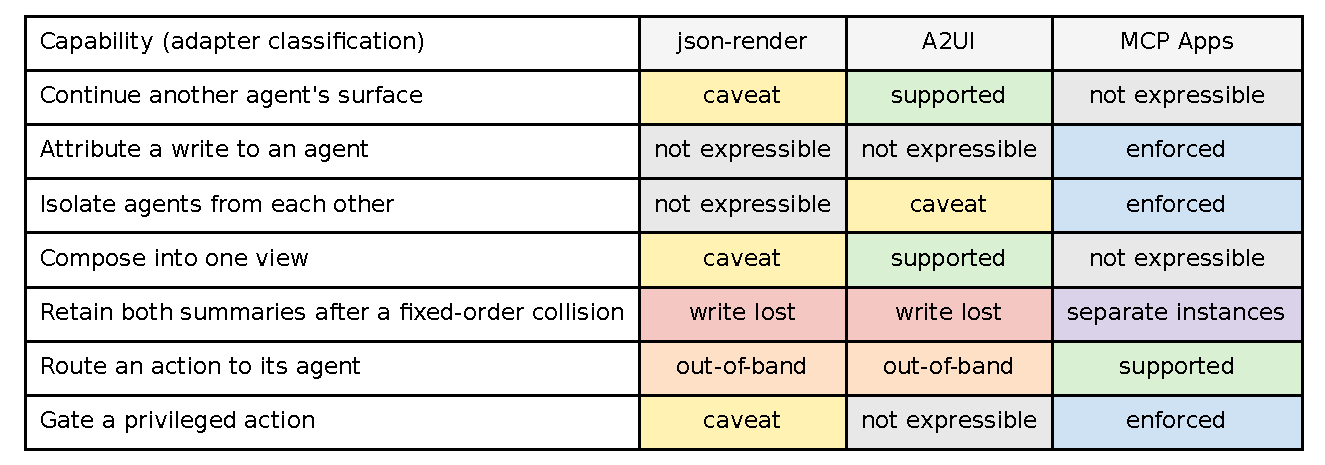
\includegraphics[width=\linewidth,height=0.70\textheight,keepaspectratio]{./figures/matrix.pdf}
\caption{Adapter-recorded classifications per capability for the three tested
configurations. Each cell is the label the adapter recorded while
driving the installed SDKs through the scripted scenarios (one retained
execution per scenario; generated from the recorded traces in
\texttt{docs/COMPARISON.md}). Labels are classifications of these
configurations, not independent measurements or protocol rankings (C8);
the collision and host-enforcement rows are backed by separate
assertions (C2, C5).}\label{fig:matrix}
\end{figure}

This empirical technical note examines three concrete tested
configurations, not three protocols in isolation. Protocol effects
cannot be separated from adapter and topology here; a matched-topology
comparison remains proposed, not performed. Its contribution is an
auditable account of a small deterministic harness: research questions,
a falsifiable hypothesis, bounded findings, an evidence map, and a local
reproduction procedure. UI descriptions, execution environments, and
authorization decisions operate at different layers; collapsing those
layers would misattribute namespace choices or host policies to a
format. The retained comparison report is an artifact to audit, not
independent scientific evidence. Scope and validity limits below delimit
the findings; no exhaustive novelty claim is made.

\section{Research questions}\label{research-questions}

RQ1: Where do the existing adapters place the output of a scripted
surface handoff?

RQ2: What survives a fixed-order identifier-collision probe in the
configured namespaces? Under the tested configurations and one fixed
write order, does reusing an identifier overwrite in the shared
json-render and A2UI mappings while being retained in separate MCP App
instances? This cannot generalize to alternative orders, scheduling or
concurrency: only the one specified sequential write order is observed.

RQ3: In the tested paths, which local bookkeeping and host decisions
determine action routing and one model-only tool rejection? In this MCP
Apps topology, originating-agent identity comes from connection binding,
not the payload.

\section{Methodology}\label{methodology}

This retrospective case study examines deterministic scripted agents,
with no LLM experiment. The unit of comparison is an SDK/adapter/host
configuration. Even uniform scenario inputs could not isolate topology,
adapter, or protocol causality. This is a bounded configuration study,
not a protocol ranking or a test of security or composition tradeoffs.
Browser MCP inputs are not identical to Node inputs. Three scenarios
exercise three configurations, with an existing permissive-host variant
for MCP Apps in S3.

\subsection{A falsifiable local
hypothesis}\label{a-falsifiable-local-hypothesis}

H1a (Node, four writes): json-render retains finance's headline and MCP
Apps retains both headlines in separate instances. H1b (browser, two
writes): A2UI's browser fixture displays finance's headline and no risk
headline within its surface; its Node check establishes only finance
writer bookkeeping. These are independent fixture-specific predictions,
not a common full-scenario browser validation. H1a and H1b observe only
the one specified sequential write order and cannot generalize to
alternative orders, scheduling or concurrency. A snapshot or DOM
assertion showing the risk headline instead of finance in a shared
summary, or loss of either isolated headline, would contradict this
hypothesis for the tested configuration.

The \href{../src/scenarios/s2-fixed-order-collision.ts}{S2 script}
awaits each emission: risk detail, finance detail, risk summary, then
finance summary. This is a fixed-order identifier-collision probe, not
actual concurrency or a scheduling benchmark. The focused check uses the
\href{../tests/protocol/scenarios.test.ts}{existing snapshot assertions}
and \href{../tests/browser/render.spec.ts}{browser assertions}, rather
than treating the adapter's \texttt{LOST} or \texttt{ENFORCED} labels as
measurements. Fresh execution status is recorded separately from this
source-based hypothesis.

\subsection{Configurations and
versions}\label{configurations-and-versions}

The \href{../package.json}{manifest} specifies ranges. The
\href{../package-lock.json}{lockfile} and locally installed package
metadata agree on the exact versions below. Package versions are not
protocol schema versions. These are observations of this checkout, not
recommendations or statements about the newest available releases.

{\def\LTcaptype{none} % do not increment counter
\begin{longtable}[]{@{}lll@{}}
\toprule\noalign{}
Configuration & Manifest range & Lockfile and installed version \\
\midrule\noalign{}
\endhead
\bottomrule\noalign{}
\endlastfoot
json-render core and React renderer & \texttt{\^{}0.21.0} each &
\texttt{0.21.0} each \\
A2UI web core and Lit renderer & \texttt{\^{}0.11.0} each &
\texttt{0.11.0} each \\
MCP Apps extension SDK & \texttt{\^{}2.0.0} & \texttt{2.0.0} \\
MCP client, core, and server & \texttt{\^{}2.0.0} each & \texttt{2.0.0}
each \\
React and React DOM & \texttt{\^{}19.2.3} each & \texttt{19.3.0} each \\
Lit & \texttt{\^{}3.3.3} & \texttt{3.3.3} \\
Zod & \texttt{\^{}4.2.0} & \texttt{4.6.5} \\
\end{longtable}
}

The A2UI adapter imports \texttt{@a2ui/web\_core/v0\_9} and emits
\texttt{version:\ "v0.9"}. Its package version \texttt{0.11.0} does not
mean that the experiment uses a v0.11 protocol. MCP Apps SDK
\texttt{2.0.0} likewise does not establish a wire protocol version. The
extension specification and SDK are separate references; no exact
upstream specification commit or negotiated wire-version value was
retained for this paper. Live repository documentation was inspected on
21 September 2026 and may differ from release-time documentation. The
local lockfile fixes the tested package resolution, not the mutable web
references.

The \href{../src/adapters/json-render/adapter.ts}{json-render adapter}
maintains one \texttt{Spec} per conceptual surface and maps logical
block, row, and control IDs to element keys. It calls
\texttt{applySpecPatch} for element additions/replacements and also
directly updates root children. Therefore, its patch log does not
capture every mutation. Its catalog validates emitted specs;
\texttt{writtenBy} is an ordinary catalog prop and \texttt{lastWriter}
is adapter bookkeeping. Neither is authenticated provenance.

The \href{../src/adapters/a2ui/adapter.ts}{A2UI adapter} validates
messages using \texttt{A2uiMessageSchema} and drives
\texttt{MessageProcessor}. Its component IDs and data paths derive from
block IDs. A shared \texttt{rootChildren} collection coordinates the
surface root. Node uses a schema-only harness catalog; the browser uses
the Lit basic catalog. Snapshot titles and writer names partly come from
adapter maps, while row values come from the data model. Surface
addressing is not authorization: an address identifies a target but does
not establish a caller's permission.

The \href{../src/adapters/mcp-apps/adapter.ts}{MCP Apps adapter} creates
one server per agent and one app instance per surface/agent pair. Its
Node path uses real SDK clients, servers, apps, and bridges connected by
in-memory transports. Its snapshot is reconstructed from adapter-held
blocks, not from a browser DOM. The \href{../web/mcp-apps.ts}{browser
host} mounts an iframe with \texttt{sandbox="allow-scripts"} for each
agent and uses \texttt{PostMessageTransport}. This topology is an
implementation choice. Connection identity is not universally agent
identity: the mapping works here because the host establishes one server
per named agent. A server could aggregate multiple agents in a different
application.

Figure \ref{fig:topology} locates the shared state, local ownership
mapping, and enforcing handler in these configurations. The dashed path
denotes the existing permissive variant, not a second enforcement
mechanism.

\begin{figure}[!htbp]
\centering

\includegraphics[width=\linewidth,height=0.70\textheight,keepaspectratio]{./figures/topology.pdf}
\caption{Configured state and enforcement boundaries. Panel A summarizes two
separate declarative-renderer runs; panel B shows the app-to-server call
path for each MCP instance. Writer maps are bookkeeping. In the tested
enforcing variant, the installed host handler rejects the model-only
call; the permissive variant forwards it. Original source-derived
illustration, not a fresh browser observation.}\label{fig:topology}
\end{figure}

\subsection{Scenario design and evidence
collection}\label{scenario-design-and-evidence-collection}

S1 opens a trip surface, emits a planner itinerary, hands off to
booking, and emits a reservation. S2 performs the fixed-order writes
specified in H1. S3 emits basket and payment controls and activates
ordinary and privileged actions. The amounts and booking operations are
fixtures: the MCP server records calls and returns text; it does not
charge money. The three scenarios are fixed examples, not a sample drawn
from a population of agent workflows.

The \href{../src/scenarios/run.ts}{runner} constructs fresh adapters per
scenario and configuration. The
\href{../src/orchestrator/orchestrator.ts}{orchestrator} is a scripted
stand-in with named agents and a control-to-agent routing table, not an
autonomous model-driven system. We inspect the existing tests and rerun
them where local prerequisites permit; no scenarios are added or their
operations or write order are modified. MCP's collision classification
records structural isolation from this adapter/topology separately from
the tested host tool-visibility handler; it does not establish a host
collision-enforcement policy.

The \href{../src/report/generate.ts}{report generator} takes
adapter-authored classifications and uses first-recording-wins selection
for each capability and configuration. It does not independently measure
the meaning of \texttt{SUPPORTED}, \texttt{SUPPORTED\_WITH\_CAVEAT},
\texttt{LOST}, \texttt{ENFORCED}, or \texttt{NOT\_EXPRESSIBLE}. Repeated
labels do not constitute independent observations. Timestamp
normalization makes its Markdown stable but does not validate its
interpretation. A freshness check establishes correspondence between
report and generator, not the truth of every sentence in the report.

We therefore distinguish classifications from assertions on snapshots,
messages, tool responses/refusals, and rendered elements. The
\href{../tests/protocol/conformance.test.ts}{conformance tests} validate
the S1 A2UI messages and json-render catalog output, examine recorded
patches, and check report and image-link freshness. They do not
establish full specification conformance. The A2UI deletion message is
not exercised in that S1 check. The json-render patch assertions do not
cover its direct root mutation.

Specifically, \texttt{Tracer.record} stores the outcome supplied by the
adapter; \texttt{outcomeOf} returns the first matching entry. In
scenario tests, json-render's S3 confirmation check and MCP's permissive
S3 check assert these labels only. MCP's S2
\texttt{SUPPORTED\_WITH\_CAVEAT}/\texttt{NOT\_EXPRESSIBLE} labels do not
measure collision prevention or impossibility of composition; the former
records structural isolation in the adapter/topology, not a tested host
collision policy. Separate assertions check the two retained headline
values. A2UI S2 checks labels and the writer map, not Node-rendered
text. The bridge tests instead exercise calls and assert actual returned
content or rejection plus refusal records. None of these labels is an
empirical score.

Browser evidence has an additional qualification: the MCP browser host
contains its own fixture script. In S2 it renders the two summaries
without the two uncontested detail blocks used by the Node scenario:
Node awaits risk-detail, finance-detail, risk/summary, finance/summary;
browser MCP awaits risk/summary, finance/summary only. Its DOM
assertions establish those browser-specific summary values, not
validation of the same full Node S2 scenario. Retained screenshots alone
cannot establish that a fresh browser run passed.

\section{Bounded observed results}\label{bounded-observed-results}

\subsection{RQ1: Handoff and placement}\label{rq1-handoff-and-placement}

Existing S1 assertions check a single \texttt{trip} snapshot region
containing both \texttt{itinerary} and \texttt{reservation} in
json-render and A2UI. MCP Apps checks separate \texttt{trip::planner}
and \texttt{trip::booking} regions. The browser assertions check both
blocks within one React tree or A2UI surface, and separate MCP iframes.
These checks support a placement observation under the chosen mappings.
They do not prove that MCP Apps cannot represent an aggregated UI or
that either declarative format provides authenticated cross-agent
ownership.

\subsection{RQ2: Fixed-order identifier
collision}\label{rq2-fixed-order-identifier-collision}

These results observe only the one specified sequential write order and
cannot generalize to alternative orders, scheduling or concurrency. The
current-source browser run verifies the fixture; earlier screenshots are
retained as historical artifacts.

The focused local S2 rerun passed its three selected tests; ten non-S2
tests in that file were skipped by the filter. The json-render assertion
checks the finance writer and headline, plus survival of the two
uncontested blocks. The A2UI Node assertion checks the finance writer
from adapter bookkeeping; its browser assertion checks headline text.
MCP snapshot assertions check both headlines in different instances. H1
has fixture-specific support from these Node checks and the canonical
current-source browser run \texttt{browser-s2-fixed-order-cFIGKT5C/} on
25 September 2026 UTC. A2UI's browser assertion checks finance's
headline visible and risk's headline absent within the surface. It does
not assert an exact summary node count, despite its test title. The
execution ledger identifies a raw browser report for the current-source
run as recording 18 passed tests: nine render assertions and nine
screenshot tests. The complete
\href{./evidence/current-browser-run/}{current browser run} resolves to
immutable \texttt{browser-s2-fixed-order-cFIGKT5C/} (25 September 2026
UTC; commit \texttt{378aabee}; Node \texttt{v23.5.0}) and includes that
report, source snapshots, build hashes, and capture hashes. The MCP
browser fixture omits Node's risk-detail and finance-detail writes. Its
two summary assertions are a separate browser result, not corroboration
of the full four-write Node S2 or support across a common shared
fixture.

Under the tested configurations and one fixed write order, reusing an
identifier overwrites in the shared json-render and A2UI mappings and is
retained in separate MCP App instances. The replacement is consistent
with reusing a slot in these shared namespaces. It is not an observed
scheduling race. The inspected adapter records a changed writer; this
trace is not an audit of all conflict signals available in a protocol or
SDK. Namespacing, ownership checks, arbitration, or shared aggregation
could change the outcome; none is evaluated as an intervention here.

Figure \ref{fig:s2} separates the four awaited writes from the retained
summary states. The arrows express script order, not elapsed time or
competing schedules.

\begin{figure}[!htbp]
\centering

\includegraphics[width=\linewidth,height=0.70\textheight,keepaspectratio]{./figures/s2.pdf}
\caption{S2 fixed-order collision: the four-write sequence is the Node fixture.
Node assertions check the json-render headline and both MCP headlines.
Executed A2UI DOM assertions check finance's headline visible and risk's
absent (C3, supported), not an exact node count. The separate MCP
browser fixture executes only risk/summary then finance/summary,
omitting both detail writes; it does not validate full Node S2. The two
MCP summaries belong to separate instances, not a merged surface. Arrows
indicate fixed script order, not time or scheduling.}\label{fig:s2}
\end{figure}

\subsection{RQ3: Routing and host
decisions}\label{rq3-routing-and-host-decisions}

In the shared-state configurations, ordinary action routing uses the
orchestrator's control table. Tests inspect routing entries and
deliveries, and the A2UI action envelope carries surface/component
fields and a timestamp without an agent field. These payload
observations do not rule out an application-supplied identity envelope.
Encoding a name in context or props would still require trusted binding
before it could authorize anything.

json-render's privileged control includes \texttt{confirm} metadata. The
Node adapter constructs an event and classifies that metadata; it does
not run an independent authorization service. The browser suite clicks
the ordinary json-render action, not the privileged confirmation flow.
Confirmation UI is not independent authorization, and the existing
assertions do not establish complete consent behavior or protection
against an omitted confirmation binding. A2UI has no privileged gate
implemented in this adapter; that is not a proof that its hosts or
trusted catalog components cannot impose one.

For MCP Apps, the \href{../src/adapters/mcp-apps/host.ts}{host} installs
one enforcing \texttt{oncalltool} handler after \texttt{bridge.connect}.
The handler looks up the tool and rejects one model-only call. The
\href{../tests/protocol/mcp-apps-bridge.test.ts}{bridge tests} check
successful app-visible calls, rejection messages and refusal records,
and successful model-only calls when enforcement is disabled. The
permissive host variant forwards that call. This is a measured
specification-versus-SDK gap for the installed enforcing host handler
and SDK-default \texttt{oncalltool}, not a security guarantee or
evidence about every MCP host or SDK release. R4 reports the external
premise that the inspected extension specification assigns visibility
enforcement to the host, but that premise is unverified within this
artifact.

Routing evidence is narrower than some trace labels suggest. For
actions, the Node MCP adapter selects the first instance for a
conceptual surface. Its helper is \texttt{findInstanceForSurface}. It
does not find the agent owning the clicked control. The routing test
only requires some delivery without the fallback table. Thus it cannot
prove correct owner routing for every S3 control. Browser S3 instead
clicks inside the cart and payments frames separately. We retain this
distinction and leave the existing behavior unchanged.

\section{Claim-evidence mapping}\label{claim-evidence-mapping}

Here \textbf{supported} means a bounded statement has a matching
inspected assertion or direct source observation, with run status
separately recorded. \textbf{Partial} means a relevant assertion exists
but leaves a material inference untested. \textbf{Proposed} means a
future check has not been performed. These terms are this paper's
evidence statuses, distinct from the adapter outcome vocabulary.

{\def\LTcaptype{none} % do not increment counter
\begin{longtable}[]{@{}
  >{\raggedright\arraybackslash}p{0.3800\dimexpr\linewidth-4\tabcolsep\relax}
  >{\raggedright\arraybackslash}p{0.1400\dimexpr\linewidth-4\tabcolsep\relax}
  >{\raggedright\arraybackslash}p{0.4800\dimexpr\linewidth-4\tabcolsep\relax}@{}}
\toprule\noalign{}
\begin{minipage}[b]{\linewidth}\raggedright
Claim
\end{minipage} & \begin{minipage}[b]{\linewidth}\raggedright
Status
\end{minipage} & \begin{minipage}[b]{\linewidth}\raggedright
Evidence and falsifier
\end{minipage} \\
\midrule\noalign{}
\endhead
\bottomrule\noalign{}
\endlastfoot
C1: S1 yields one shared region or two MCP instances in this topology. &
Supported & S1 snapshot region and block assertions; contradicted by
missing blocks or different region counts. \\
C2 / H1a (Node, four writes): Under the tested configurations and one
fixed write order, reusing an identifier overwrites in the shared
json-render and A2UI mappings and is retained in separate MCP App
instances. & Supported & Node headline assertions; contradicted by
different retained values. The browser fixture is not evidence for
H1a. \\
C3 / H1b (browser, two writes): Under the tested A2UI shared mapping and
fixed write order, the fixture displays finance's headline after the
later write. & Supported & The cited
\href{./evidence/current-browser-run/}{current browser run} resolves to
immutable \texttt{browser-s2-fixed-order-cFIGKT5C/} (25 September 2026
UTC; commit \texttt{378aabee}; Node \texttt{v23.5.0}) and records
assertions checking finance visible and risk absent within the surface.
It is distinct from H1a and does not assert an exact node count. \\
C4: S2 is sequential, with no scheduling test. & Supported & Four
awaited emissions in the S2 source; contradicted by an overlapping
scheduler in the executed path. \\
C5: The enforcing MCP handler rejects the model-only call, while the
permissive variant forwards it. & Supported & Bridge rejection/refusal
and successful-result assertions; contradicted by reversed or identical
behavior. \\
C6: Every MCP S3 control reaches its intended agent. & Partial &
Existing test checks some table-free delivery; first-instance selection
prevents this stronger inference. \\
C7: json-render includes confirmation metadata, with consent enforcement
incompletely checked. & Partial & Adapter source includes metadata; the
scenario test asserts its classification only, not independent policy or
privileged browser consent. \\
C8: Matrix labels are adapter classifications, not independent
measurements. & Supported & Source shows adapter-authored
classifications; freshness checks correspondence only. \\
C9: A matched-topology intervention isolates protocol causality. &
Proposed & Pending controlled comparison; no new experiment is reported.
The one-server-per-agent topology has not been ablated, so no collision,
isolation, or host-policy result is protocol-level. All collision
findings are conditioned on the one fully deterministic write order and
cannot be extrapolated to concurrent or out-of-order writes. \\
\end{longtable}
}

Each \textbf{Supported} row reflects exactly one retained execution
(n=1) identified for its check; the harness uses deterministic scripted
agents rather than an LLM experiment. No mean, variance, pass rate, or
run-to-run browser stability is claimed.

The linked scenario, bridge, conformance, and browser test files in
Methodology and Results are the check locations for C1--C8. This mapping
exposes uneven coverage rather than assigning a numeric score across
unlike checks.

For C1--C3 and the tested browser actions, the renamed
\href{../tests/browser/render.spec.ts}{render spec} supplies the
assertions and the
\href{../tests/browser/screenshots.spec.ts}{screenshot spec} supplies
nine captures. By contrast, the earlier pre-rename
\texttt{browser-terminal-20260922T013449Z-zH4HTK/} records are
historical only and are not claim-support evidence for this fixture. The
execution ledger records the single cited
\href{./evidence/current-browser-run/}{current browser run}, which
resolves to immutable \texttt{browser-s2-fixed-order-cFIGKT5C/} (25
September 2026 UTC; commit \texttt{378aabee}; Node \texttt{v23.5.0}).
Its report, source snapshots, build hashes, and capture hashes bind the
current browser claim for this fixture. Other retained browser
directories have different source snapshots and are execution records,
not redundant confirmation of this claim. This does not make the
distinct MCP browser fixture corroborate the four-write Node fixture. C6
remains partial: successful browser actions in its distinct fixture do
not repair the Node first-instance routing gap.

\section{Related work}\label{related-work}

The json-render repository describes catalog-defined components and
actions rendered from structured specifications {[}R1{]}. A2UI similarly
separates declarative UI data from client implementation and describes a
trusted component catalog {[}R2{]}. These are meaningful security
properties: constraining requested components and handlers can limit
what untrusted UI data asks the client to run. They do not by themselves
establish per-writer authorization in our shared namespace. Conversely,
our collision example is not evidence of blanket insecurity in
declarative rendering.

The MCP Apps repository describes tool-associated UI resources and a
host bridge {[}R3{]}. Its specification describes visibility checks and
sandbox/CSP obligations {[}R4{]}. Those obligations are not proof that
this harness checks all of them. In particular, iframe sandbox
attributes and successful bridge tests do not establish exhaustive CSP
enforcement, transport security, or resistance to malicious content.
Declarative catalogs and sandboxed app delivery are compatible layers: a
hosted application could use a declarative renderer internally. No
integration experiment is reported here.

The claim-status vocabulary is defined in this paper's Claim-evidence
mapping: it separates an inspected assertion or direct source
observation from a material untested inference and from a proposed
future check. It does not depend on an unavailable external
methodological source. This discussion is selective, not an exhaustive
literature or novelty review.

\section{Threats to validity}\label{threats-to-validity}

\textbf{Internal validity.} Identical logical inputs leave adapter
bookkeeping, shared-root coordination, naming conventions, host
enforcement, catalogs, rendering frameworks, transports, and
one-server-per-agent MCP topology as confounders. The default/permissive
MCP comparison narrows one host-policy question, but it is not a
factorial comparison across all configurations. Accordingly, the
isolation and collision findings describe the tested adapter and
topology configurations, not protocol-level enforcement results; a
matched-topology intervention remains unperformed.

\textbf{Construct validity.} A region count is a property of the adapter
snapshot; it is not a usability measure. A writer prop is not
authenticated provenance. Addressability is not authority. A
confirmation binding is not an authorization decision. Adapter labels
and some scenario assertions share their interpretation, creating a risk
of circular validation. The editorial and manuscript regression tests
are likewise authored and iteratively adjusted by the same AI-assisted
process that produced the prose they check. The independent aspects of
the checks are the inspected contents, response/refusal assertions, and
DOM expectations; they are still authored within this repository, not by
independent evaluators.

\textbf{Execution and coverage.} Node transports do not test browser
isolation. The MCP browser fixtures differ from the Node scenario.
Historical screenshots remain retained artifacts; the nine new captures
are separately archived and do not establish historical reproduction.
Four post-rename attempts are retained: two completed with 18 passing
tests, and two aborted before any test body ran. The two completed
executions used different source revisions: their snapshots differ for
\texttt{src/adapters/mcp-apps/adapter.ts},
\texttt{src/orchestrator/types.ts}, and \texttt{src/report/generate.ts}.
Each reported pass count is from one execution (n=1), not repeated
trials; no mean, variance, or stability statistic is claimed. No
per-test timing or other run-level equivalence is claimed. No completed
execution was discarded, and the immutable current-source run is
\texttt{paper/evidence/browser-s2-fixed-order-cFIGKT5C/} (25 September
2026 UTC; commit \texttt{378aabee}; Node \texttt{v23.5.0}). Neither
completed run is an independent reproduction: both ran on the same
machine, from the same checkout, in the same session. No adversarial,
forged-identity, CSP, or cross-server test was run. The suite also does
not comprehensively test transport authentication, authorization
revocation, or arbitrary concurrent schedules. No completed security
review is claimed.

\textbf{Classification scope.} The matrix contains many individually
classified configuration/scenario cells. Because these are deterministic
code-behavior observations rather than independent statistical tests, no
multiple-comparison estimate is reported. The number of cells
nevertheless increases the surface for a stale or incorrect
classification; the freshness check tests report/code correspondence,
not the truth of every classification.

\textbf{External and temporal validity.} Three designed scenarios, fixed
fixture data, and the pinned installed packages cannot establish
population effects or general protocol superiority. Later SDKs, other
renderers, different server topologies, and stricter application
policies can behave differently. Mutable upstream documentation is
contextual evidence, not a version-pinned release archive. No latency,
throughput, cost, user study, or model capability was measured.

\section{Data availability}\label{data-availability}

The exact evidence reported here is archived as v0.2.0 at
https://doi.org/10.5281/zenodo.22965404. The concept DOI,
https://doi.org/10.5281/zenodo.22896881, resolves to the latest version.
The archive contains the harness, the editable manuscript, a frozen v0.1
Markdown snapshot, and the versioned evidence records cited in this
paper. The harness code is released under the Apache License 2.0; the
manuscript, figures and evidence records under CC BY 4.0, as identified
by the root \texttt{LICENSE} and package metadata.

\section{Reproducibility}\label{reproducibility}

The \href{./REPRODUCTION.md}{reproduction guide} gives commands and
expected semantic outcomes, and the \href{./EXECUTION.md}{execution
record} lists every command run, including failed attempts and
unavailable prerequisites, with retained artifacts. Inputs, tooling, and
evaluation configuration are versioned now; commit-level provenance
before 22 September 2026 does not identify the complete paper workspace.
Separate paper checks and SHA-256 manifests record the manuscript,
tooling, figures, and generated outputs.

Semantic reproducibility means obtaining the specified regions, values,
events, and refusal behavior under the same configuration. Byte identity
is a separate question. A2UI action timestamps vary; report generation
normalizes those timestamps. We check generated LaTeX against fresh
Pandoc output under the recorded toolchain, not PDF byte identity across
machines. The Markdown manuscript is the only editable paper source;
LaTeX and PDF are generated derivatives.

The Node test suite (24 tests across three files) and TypeScript
checking pass. The browser claims rest on the
\href{./evidence/current-browser-run/}{current browser run}, which
resolves to immutable \texttt{browser-s2-fixed-order-cFIGKT5C/} (25
September 2026 UTC; commit
\texttt{378aabee42a69c61edc7d7a37c934465b4a66e30}; Node
\texttt{v23.5.0}) and records current-source and build hashes, 18
passing tests, and nine capture hashes. All runs were performed on a
single machine by the author; independent reproduction has not been
performed.

\section{Conclusion}\label{conclusion}

S2 observes only the one specified sequential write order and cannot
generalize to alternative orders, scheduling or concurrency. The
retained pre-rename browser findings are historical; the complete
\href{./evidence/current-browser-run/}{current browser run}, resolving
to immutable \texttt{browser-s2-fixed-order-cFIGKT5C/} (25 September
2026 UTC; commit \texttt{378aabee}; Node \texttt{v23.5.0}), supplies
current browser-source provenance for the renamed fixture.

Across three concrete tested configurations, handoff placement and
retained values reflect the chosen shared or separated mappings. Under
the tested configurations and one fixed write order, reusing an
identifier overwrites in the shared json-render and A2UI mappings and is
retained in separate MCP App instances. Node assertions establish the
four-write S2 outcome for those configurations. Browser MCP executes
only risk/summary then finance/summary. Those browser observations
corroborate rendered outcomes only for their own fixtures and cannot
validate the Node four-write fixture. Neither fixture tests concurrency,
scheduling, interleaving, or randomization. MCP model-only tool
rejection is measured behavior of one installed enforcing host handler,
whereas SDK-default \texttt{oncalltool} forwards it; this is a
specification-versus-SDK gap, not a security guarantee. In the tested
topology, originating-agent identity comes from connection binding
rather than the payload, while correct routing for every control remains
only partially checked. Protocol effects cannot be separated from
adapter and topology here; a matched-topology comparison remains
proposed, not performed. These results do not isolate protocol
causality, establish protocol-level collision enforcement, or establish
unavoidable incompatibility between composition and security. No
adversarial, forged-identity, CSP, or cross-server test was run.
Integrations remain possible, and trusted catalogs retain meaningful
security properties.

Future experiments are explicitly pending: matched namespaces and
topology, controlled scheduling with overlapping writes, trusted
identity envelopes, privileged confirmation interaction tests, and
complete host-policy tests. They are suggestions for separate approved
work, not results of this paper.

\section{AI-assistance disclosure}\label{ai-assistance-disclosure}

An OpenAI Codex coding assistant inspected local source and accessible
references, assisted with drafting and editorial revision, prepared
source-derived figures and supporting documentation, added focused
manuscript checks, and executed the recorded local validation commands.
Anthropic Claude assisted with editorial revision. The author reviewed
all claims, citations, limitations, and the final presentation, and
takes full responsibility for the content. AI-assisted preparation is
separate from the deterministic harness: no LLM participates in its
scenario runs.

\section{References}\label{references}

R1. Vercel Labs.
\href{https://github.com/vercel-labs/json-render/tree/3ad381881194e7011ad3ccd6d668033495a06c29}{json-render
repository and README}. Inspected 21 September 2026 at commit
\texttt{3ad381881194e7011ad3ccd6d668033495a06c29}. Local SDK context:
\texttt{@json-render/core} and \texttt{@json-render/react} 0.21.0. Used
for catalog/renderer design, not a security proof.

R2. A2UI project.
\href{https://github.com/a2ui-project/a2ui/tree/c08702a4bf8ab22a862cf5de8b5b1542be6081f6}{A2UI
repository and README} (the inspected \texttt{google/A2UI} URL redirects
here). Inspected 21 September 2026 at commit
\texttt{c08702a4bf8ab22a862cf5de8b5b1542be6081f6}. Local context: web
core and Lit 0.11.0, and the adapter-selected v0.9 schema.

R3. Model Context Protocol contributors.
\href{https://github.com/modelcontextprotocol/ext-apps/tree/6d9bdc7babf275b759225aa722cbf5510c4c6021}{MCP
Apps SDK repository and README}. Inspected 21 September 2026 at commit
\texttt{6d9bdc7babf275b759225aa722cbf5510c4c6021}, the same revision R4
pins. Local context: extension, client, core and server packages 2.0.0.
SDK package version is distinct from wire version.

R4. Model Context Protocol contributors.
\href{https://github.com/modelcontextprotocol/ext-apps/blob/6d9bdc7babf275b759225aa722cbf5510c4c6021/specification/draft/apps.mdx}{MCP
Apps extension specification, draft/apps.mdx}. Visibility and
sandbox/CSP sections inspected 21 September 2026; source path pinned to
commit \texttt{6d9bdc7babf275b759225aa722cbf5510c4c6021}. The pin was
added after earlier retained evidence used a mutable main path; this
document records the pin but does not include an archived copy or
independent verification of it. Its reported host-requirement premise is
therefore unverified within this artifact and is not evidence for the
host-enforcement conclusion. The filename's ``draft'' is retained as the
source location, without claiming a release status from the SDK version.
\end{document}
